\section{Method}
In this section the methodology is covered in four parts.
First the practical procedure chosen in this work for applying \spectral{} is given.
Secondly, choices and interpretations for the variable parameters in this algorithm are given.
Then the datasets against which this will be measured are specified.
Finally the procedure for checking infrared-collinear (IRC) safety will be described.


\subsection{Clustering algorithm}\label{sec:spectralmethodalgo}
    The implementation of the theory described in section~\ref{sec:spectral_theory} will be specified.
    For every simulated event this process is used to identify the jets.

    To begin, relevant cuts are applied to the particles to simulate the detectors reconstruction capability.
    These are described in section~\ref{sec:particle_data}.
    Then all particles are declared pseudojets, and given an index, \(j = 1 \dots n\), with no particular order.
    The algorithm is recursive and agglomerative, and the first time step is labelled \(t=1\).

    \begin{enumerate}
        \item \label{step:start} The pseudojets are used to form the nodes of a graph,
        the edges of which will be weighted by some measure of proximity between the particles called affinity.
        To obtain an affinity, first a distance is obtained.
        Between pseudojets \(i\) and \(j\) this would be \(d(t)_{i,j} = \sqrt{(y(t)_i - y(t)_j)^2 + (\phi(t)_i - \phi(t)_j)^2}\)
        where \(y(t)_j\) is the rapidity of pseudojet \(j\) at time step \(t\) and \(\phi(t)_j\) is the barrel angle, likewise for \(i\).
        No \(p_T\) dependence is used.

    \item \label{step:affinity} The affinity must increase as pseudojets become more similar, whereas the distance will shrink.
        This is done by taking an exponent so that \(a(t)_{i,j} = \text{exp}(-d(t)_{i,j}^\alpha/\sigma_v)\), as done in~\cite{hadjighasem2016votex}.
            Distances much larger than \(\sigma_v\) are only allowed very small affinities,
            thus less influence over the clustering.

    \item\label{step:KNN} The affinity between pseudojets that are far apart contains less useful information,
        such pseudojets are unlikely to be good combinations.
        Removing these affinities reduces noise.
    A fixed number, \(k_\text{NN}\), of neighbours of each pseudojet are
    preserved, and all other affinities are set to zero.
    Thus in a group with more than \(k_\text{NN}\) pseudojets,
    each pseudojet has at least \(k_\text{NN}\) non zero affinities with other pseudojets.

\item\label{step:laplacean} These affinities allow the construction of a Laplacian.
    The Laplacian used is the symmetric Laplacien, which is proportional to \(-a(t)_{i, j}\)
        in the \(i\)th row and \(j\)th column, and exactly \(1\) on the diagonal.
        For ease of notation let \(z(t)_j\) be a measure of the size pseudojet \(j\) contributes to a cluster,
        with \(z(1)_j = \sum_k a_{i,k}\).
        The laplacian can now be written;
    \begin{equation}\label{eqn:laplacian}
        L(t) = 
        \begin{pmatrix}
            z(t)_1      & 0   & 0  & \hdots \\
            0     & z(t)_2 &    0     & \\
            0     &    0     & z(t)_3 & \\
            \vdots   &          &     & \ddots 
        \end{pmatrix}^{-\frac{1}{2}}
        \begin{pmatrix}
            z(t)_1 & -a(t)_{1,2} & -a(t)_{1,3} & \hdots \\
            -a(t)_{1,2} & z(t)_2 & -a(t)_{2,3} & \\
            -a(t)_{1,3} & -a(t)_{2,3} & z(t)_3 & \\
            \vdots   &          &     & \ddots 
        \end{pmatrix}
        \begin{pmatrix}
            z(t)_1      & 0   & 0  & \hdots \\
            0     & z(t)_2 &    0     & \\
            0     &    0     & z(t)_3 & \\
            \vdots   &          &     & \ddots 
        \end{pmatrix}^{-\frac{1}{2}}.
    \end{equation}
        When two pseudojets are combined, instead of calculating \(z_j\) as the sum of the affinities of the combined pseudojet,
        the new \(z_j\) is the sum of the two previous \(z_j\).
        For example, if pseudojet \(1\) and \(2\) from \(t=1\) are to be combined to make pseudojet \(1\) in \(t=2\),
        then \(z(2)_{1} = z(1)_1 + z(1)_2\) rather than the sum of affinity between new pseudojet \(1\) and other pseudojets in step \(t=2\).
        This condition is required for IRC safety.  % TODO add some discussion/proof

    \item \label{step:eigenvectors} From the Laplacian eigenvectors are calculated to create the embedding space, and labelled with index \(q\).
            \begin{equation}
                L(t)h_q(t) = \lambda_q(t) h_q(t)
            \end{equation}
            All non-trivial eigenvectors, corresponding
            to an eigenvalue less that the eigenvalue limit, \(\lambda_q(t) < \lambda_\text{limit}\),
            are retained.
            Then the index runs over \(q = 1 \dots c\).
            See section~\ref{sec:eig_norm} for discussion.

        \item \label{step:compression} Eigenvector is divided by the corresponding eigenvalue raised to \(\beta\)
            This acts to compress the dimensions that hold less information, again see section~\ref{sec:eig_norm}.
            The embedding space can now be formed.
            The eigenvectors have as many elements as there are pseudojets, and the coordinates of
            the \(j^\text{th}\) pseudojet at time step \(t\)
            become \(m(t)_j = \left(\lambda_1(t)^{-\beta} h_1(t)_j, \dots \lambda_c(t)^{-\beta} h_c(t)_j\right)\).
            The first embedding space of a clustering is shown in figure~\ref{fig:embedding_space_simple}.

        \item  A measure of distance between all pseudojets in the embedding space is calculated.
            In the embedding space angular distances are most appropriate, see section~\ref{sec:embedding_distance}.
            \begin{equation}
                d'(t)_{i, j} = \text{arccos}\left|\frac{m(t)_i.m(t)_j}{{||m(t)_i||}_2 {||m(t)_j||}_2}\right|
            \end{equation}

        \item\label{step:stoppingcondition}

            Provided the mean of this distance is less than \stoppingdeltar{}, that is;
            \begin{equation}
                \frac{1}{c}\sum_{i\ne j} d'(t)_{i, j} < \stoppingdeltar{}
            \end{equation}
            then the two pseudojets that have the smallest embedding distance are combined.
            Reasons for this stopping condition are given in section~\ref{sec:stopping_condintion}.
        The two pseudojets that have been combined are removed and replaced with one pseudojet.
        In physical space the new pseudojet is created by summing the respective four momenta of the removed pseudojets.
        Once two pseudojets have been combined in physical space, the embedding space is recalculated from step~\ref{step:start}, 
        to begin time step \(t+1\).
        There will be one fewer row and column in the Laplacian of step \(t+1\).
    \end{enumerate}

    When the mean of the distances in the embedding space rises above \stoppingdeltar{},
    then all remaining pseudojets are promoted to jets.
    Jets with less than 2 tracks are removed, and their contents considered noise.
    Further cuts may then be applied as described in section~\ref{sec:particle_data}.

    These steps will form a variable number of jets from a variable number of particles.
    An example of the constructed embedding space is shown in figure~\ref{fig:embedding_space_simple}.
    This illustrates how the embedding space highlights the clusters.

    \begin{figure}[htp]
        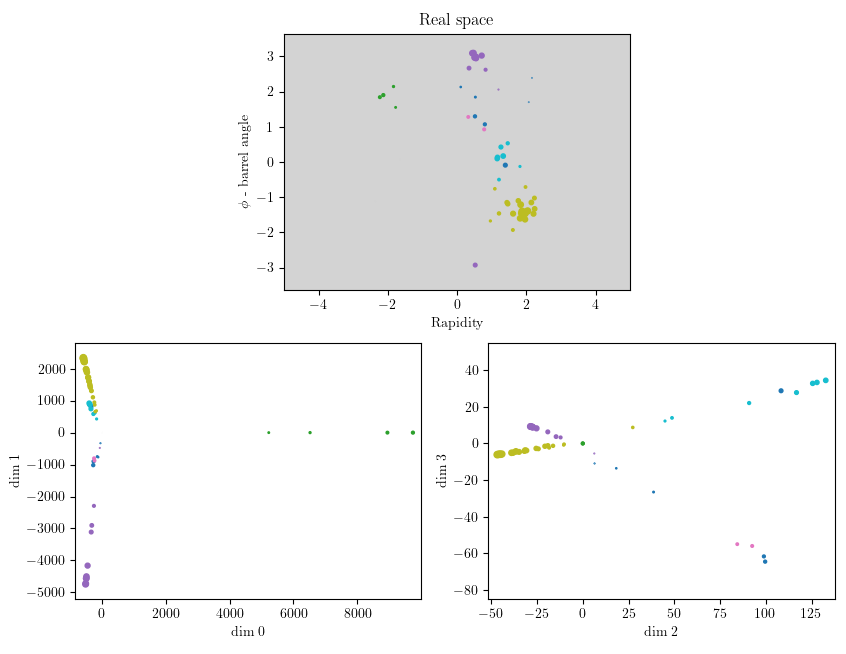
\includegraphics[width=1\textwidth]{graphics/embedding_space_simple.png}
        \caption{A single event and it's embedding space, as created by \spectral{}.
            At the top the grey plot shows the particles in the event as points on the unrolled detector barrel.
            The colour of each point indicates the shower it came from.
            The lower two plots show the first 4 dimensions of the embedding space,
            and the location of the points within the embedding space.
        }\label{fig:embedding_space_simple}
    \end{figure}    

    %To provide a basis for comparison the results of clustering with an \antikt{}  algorithm (as in~\cite{Cacciari2008akt}) is also shown.

\subsection{Tunable parameters}\label{sec:spectralmethodparam}
Unlike most machine learning techniques, \spectral{} does not have large arrays of learnt parameters.
The parameters for the clustering are a small, interpretable, set.
Appropriate values were chosen by performing scans and observing the influence of changes to the parameters on jets formed.

In section~\ref{sec:spectralmethodalgo} 5 parameters are named;
\(\sigma_v\), \(\alpha\), \(k_\text{NN}\), \(\lambda_\text{limit}\), \(\beta\) and \stoppingdeltar{}.
These parameters have a range of values for which sensible results are obtained.
The interpretation of these parameters is given here;
\begin{itemize}
    \item \(\sigma_v\); introduced in step~\ref{step:affinity}, this is a scale parameter in physical space.
                      The value indicated an approximate average distance for particles in the same shower,
                      or alternatively, the size of the neighbourhood of each particle.
                      It is closely tied to the stopping parameter for the \genkt{} algorithm, \ktstoppingdeltar{},
                      they both relate to the width of the jets formed.
                      It should take values on the same order of magnitude as \ktstoppingdeltar{}, \(\mathcal{O} (0.1)\).
    \item  \(\alpha\); also introduced in step~\ref{step:affinity},
           this changes the shape of the distribution used to describe the neighbourhood of a particle.
           Higher values make the probability of joining particles outside \(\sigma_v\) fall away faster.
           Traditionally the value used here is \(2\), like in a Gaussian distribution.
       \item \(k_\text{NN}\); introduced in step~\ref{step:KNN}, this dictates the minimum number of non-zero affinities around each point.
           Lower values create a sparser affinity matrix, reducing noise at the potential cost of lost signal.
           Values above \(7\) are seen to have to have little impact.
       \item  \(\lambda_\text{limit}\); introduced in step~\ref{step:eigenvectors}, is a means of limiting the number of eigenvectors used
           to create dimensions in the embedding space.
           Only eigenvectors corresponding to eigenvalues less than \(\lambda_\text{limit}\) are used.
           Thus the number of dimensions in the embedding space can be increased with a larger \(\lambda_\text{limit}\),
           however, as the eigenvalues will be influenced by the number of clear clusters available 
           there will not be the same number of dimensions in each event.
           This is discussed in section~\ref{sec:eig_norm}.
           For a symmetric Laplacian the eigenvalues are \(0 < \lambda < 2\)
           so values \(\mathcal{O} (0.1)\) are sensible choices.
       \item  \(\beta\); is introduced in step~\ref{step:compression}.
           To account for variable quality of information in the eigenvectors, as given by their eigenvalues,
        dimensions of the embedding space with lower quality information are compressed.
        The larger the value of \(\lambda_\text{exponent}\) the more dimensions with lower quality information are compressed.
        This is discussed in section~\ref{sec:eig_norm}.
%        This is should be \(\mathcal{O}(1)\).
    \item \stoppingdeltar{}; is introduced in step~\ref{step:stoppingcondition}.
         This determines the expected spacing between jets, in the embedding space.
         As the number of dimensions in the embedding space grows with increasing 
         number of clear clusters it will not result in the same or
         similar number of clusters each time.

\end{itemize}


%A number of other parameters that could influence clustering were experimented with,
%including changed of Laplacian and parameters using \(p_T\).
%These modifications did not seem to improve performance, so they are not included.

To investigate the behaviour of the clustering when the parameters change scans where performed.
On a small sample of events (\(2\)k events) the clustering is performed with many different parameter choices.

With the aid of MC truth information a metric of success can be created.
For each object we wish to find (e.g. a \bthing{quark}) 
the MC truth can reveal which of the particles that are visible to the detector have
been created by that object.
In many cases, a particle see in the detector will have been created by two objects,
such as a particle coming from an interaction between a \(b-\bar{b}\) pair,
in these cases both objects are considered together.
The complete set of visible particles that came from these objects could be referred to as their descendants.
The aim in jet clustering is to capture only all of the descendants in the same number of jets as there were objects that created them.
So the descendants of \(b-\bar{b}\) pair should be captured in exactly 2 jets.

There are two ways a jet finding algorithm can make mistakes in this task:
the first is to omit some of the descendants of the objects being reconstructed, causing the jet to have less mass than it should;
the second is to include particles that are not in the descendants of the objects being reconstructed, such as initial state radiation or particles from other objects,
causing the jet to have more mass than it should.
The effects of these mistakes will cancel in the jet mass,
but they are both still individually undesirable,
so separate metrics are made for each of them.
The first is ``Signal mass lost", the difference between the mass of the jets and the mass they would have had if all they contained all descendants of the object being reconstructed.
The second is ``Background contamination", the difference between the mass of jets and the mass they would have if they didn't contain anything but descendants of the objects being reconstructed.
The standard algorithm for this process, the \antikt{} algorithm with \(\stoppingdeltar{}_\text{kt}=0.8\), slightly prefers suppressing ``Signal mass lost" over ``Background contamination",
this leads to the clearest mass peaks.
When the metrics are combined into a single loss value this is accounted for by weighting;
\begin{equation}\label{eqn:loss}
\text{Loss} = \sqrt{0.73(\text{Background contamination})^2 + (\text{Signal mass lost})^2}
\end{equation}

An example of this scan for the \genkt{} algorithm is given in figure~\ref{fig:scan_genkt}.
For \spectral{} there are more than 2 variables to deal with, 
so a set of two dimensional slices are shown in figure
These slices have been chosen to include the best performing combination.
    \begin{figure}[htp]
        \begin{minipage}[c]{0.5\textwidth}
            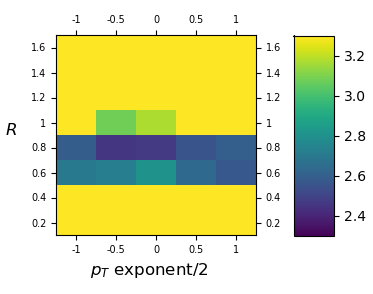
\includegraphics[width=1\textwidth]{graphics/trangle_scan_genkt.png}
        \end{minipage}\hfill
        \begin{minipage}[c]{0.45\textwidth}
            \caption{The \genkt{} algorithm offers two parameters that can be varied.
                The stopping condition, \ktstoppingdeltar{}, and a multiple for the exponent of the \(p_T\) factor.
                When the exponent of the \(p_T\) factor is \(-1\) the algorithm becomes the \antikt{} algorithm.
                Here the loss, as described in equation~\ref{eqn:loss}, is shown for a number of parameter combinations.
                It can be seen that while good results are possible with many values of \(p_T\) exponent,
                \ktstoppingdeltar{} must fall in a narrow range to yield good results.
             }\label{fig:scan_genkt}
        \end{minipage}
    \end{figure}    

    \begin{figure}[htp]
            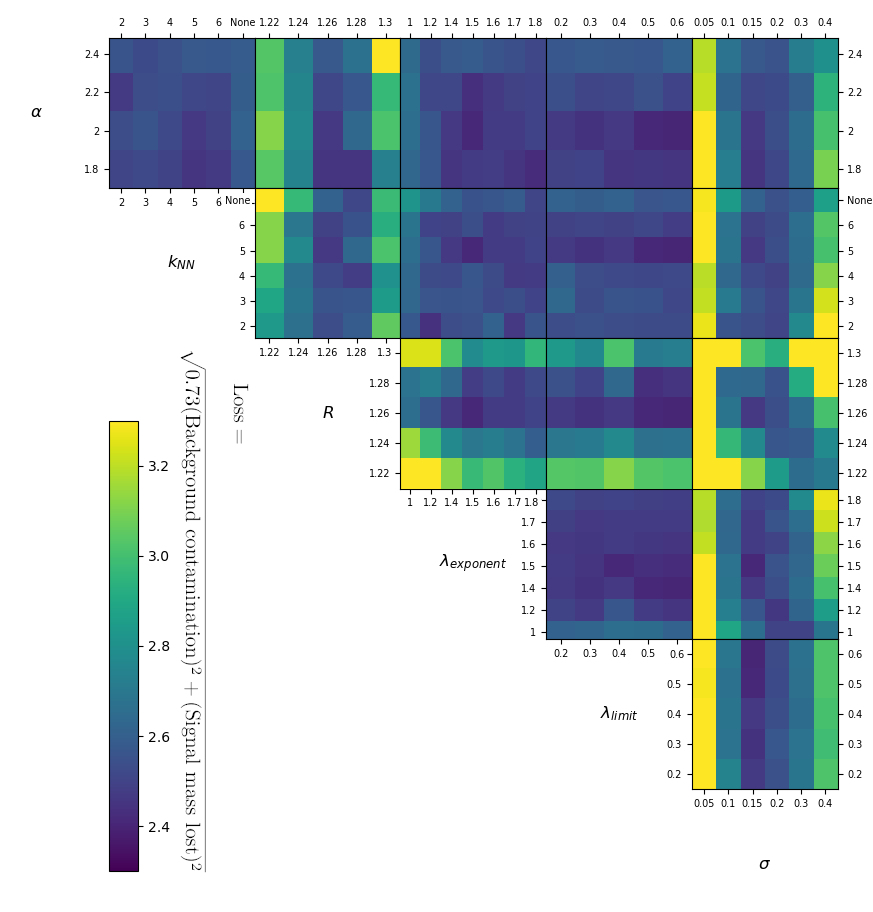
\includegraphics[width=1\textwidth]{graphics/trangle_scan_incomplete.png}
            \caption{There are 5 free parameters for \spectral{},
                as described in section~\ref{sec:spectralmethodparam}.
                Here the loss, as described in equation~\ref{eqn:loss}, is shown for reasonable of parameter ranges.
                These ranges are either chosen by convention (e.g. \(\alpha\) is conventionally \(1\) or \(2\))
                or chosen according to physical scales (e.g. the distance between particles is of order \(0.1\),
                so \(\sigma\) should be of the same order).
                It can be seen that some parameters, such as \(\alpha\), \(k_\text{NN}\), \(\lambda_\text{exponent}\)
                and \(\lambda_\text{limit}\) are relatively insensitive.
                They give good results in a wide range of values.
                By contrast \stoppingdeltar{} and \(\sigma\) must fall in a narrow range to yield good results.
             }\label{fig:scan_spectral}
    \end{figure}    

    As can be seen in figure~\ref{fig:scan_spectral}, the parameters choices of \spectral{} are not finely tuned.
    Unlike the \antikt{} algorithm, there is flexibility in all parameter choices.
    The parameters used in the remained of this work are \(\alpha=2.\), \(k_\text{NN}=5\), \(\stoppingdeltar{} = 1.26\), \(\lambda_\text{exponent} = 1.4\), \(\sigma = 0.15\) and \(\lambda_\text{limit} = 0.4\).
    \subsection{Particle data}\label{sec:particle_data}

    In order to evaluate the behaviour of this clustering method four datasets are used.

    \begin{enumerate}
        \item A \(125\)GeV simulated \textbf{light Higgs cascade decay}.
    One Standard Model (SM) Higgs at \(125\)GeV decays to two light Higgs at \(40\)GeV,
    which in turn decay to \beau{}-\bbar{} quark pairs.
    That is \(p^+ p^+ \rightarrow H_{125\text{GeV}} \rightarrow h_{40\text{GeV}} h_{40\text{GeV}} \rightarrow \beau \bbar \beau \bbar\).

\item The second dataset used is a \(500\)GeV simulated \textbf{heavy Higgs cascade decay}.
         One Heavy Higgs, from the two Higgs doublet model, type-II~\cite{2hdm_modelfile}, at \(500\)GeV decays to two SM Higgs at \(125\)GeV,
    which in turn decay to \beau{}-\bbar{} quark pairs.
    That is \(p^+ p^+ \rightarrow H_{500\text{GeV}} \rightarrow h_{125\text{GeV}} h_{125\text{GeV}} \rightarrow \beau \bbar \beau \bbar\).

\item To obtain jets with a different width, a \textbf{semileptonic top decay} is used.
        That is \( p p \rightarrow t \bar{t} \rightarrow W^+ b W^- \bar{b} \)  where one \(w\) decays to a pair of quark jets, and the other decays leptonically.
        The quark jets from the \(w\) may be \(u\), \(c\), \(d\), \(s\) or \(b\).
        

    \item For the purpose of checking \textbf{IRC safety} a variety of three jet events are used.
        These jets can be created by any combination of \(g\), \(u\), \(c\), \(d\), \(s\), and their antiparticles.
        It will be generated at leading order and next to leading order.
        This being the simplest possible configuration where IRC singularities could be observed.

    \end{enumerate}

    Using Madgraph~\cite{alwall_madgraph2011} to generate the partonic process, and Pythia~\cite{sjostrand_pythia2015} to shower, ${\cal O}(10^5)$ of each of these processes are generate.
    The center of mass energy used is \(\sqrt{s}=13 \) TeV.


    Both Higgs cascade datasets have the desirable property of creating \bthing{jets} with a range of geometries,
    owing to the boost provided by large mass difference,
    there is a high chance of overlap with 4 \bthing{quarks} in the event.

    Each event also contains some initial state radiation (ISR),
    and from beam remnants.
    ISR is other emissions from the quarks that create the signal process,
    such as radiated gluons.
    Beam remnants are emissions coming from the part of the proton that is not directly involved
    in creating the signal process.


    Each of these datasets requires different cuts,
    both at the reconstructed particle level to simulate detector accuracy,
    and at the jet level, to select the best reconstructed events.
    The cuts of each dataset are;
    \begin{enumerate}
        \item \textbf{Light Higgs cascade decay}; The reconstructed particles are required to have
            rapidity \(< 2.5\) and \(p_T > 0.5\) GeV.
            These cuts are likely to remove the majority of the radiation from beam remnants,
            and reduce the radiation from ISR.
            After cuts, \(72\%\) of events have at least \(5\) \bthing{shower} particles and \(5\) pure ISR shower particles available.
            The jets are required to have \(p_T > 15\) GeV, which is lower than is realistic,
            but leaves a larger range of events to compare the behaviour of jet clustering algorithms.
        \item \textbf{Heavy Higgs cascade decay}; The reconstructed particles are required to have
            rapidity \(< 2.5\) and \(p_T > 0.5\) GeV.
            The jets are required to have \(p_T > 30\) GeV, which is realistic.
            
        \item \textbf{Semileptonic top decay}; The reconstructed particles are required to have
            rapidity \(< 2.5\) and \(p_T > 0.5\) GeV.
            The event is required to have at least \(p_{T,\text{miss}} > 50\) GeV,
            where \(p_{T, \text{miss}}\) is the missing transverse momentum due to 
            the neutrino.
            The lepton in the event must have rapidity \(< 2.4\).
            If the lepton in the event is a muon then its \(p_T\) must be \(>  55\) GeV.
            If the lepton in the event is an electron and it is isolated (as defined in~\cite{Sirunyan_2018}) then its \(p_T\) must be \(> 55\), if it is not isolated then \(p_T > 120\).
            The reconstructed jets must have \(p_T > 30\) and rapidity \(< 2.4\).
            Finally, the lepton must be seperated from the closest jet by at least
            \(\sqrt{\Delta \text{rapidity}^2 + \Delta \phi^2} > 0.4\) or
            \(p_{T, \text{relative}} > 40\) GeV.
            These cuts are copied from~\cite{Sirunyan_2020}.
        \item \textbf{IRC safety}; the only restriction on the particles is that rapidity must be \(< 2.5\).
            There are no cuts on the jets.
            Issues of IRC safety are emphasized at low \(p_T\), so to highlight this we abandon all \(p_T\) cuts.

    \end{enumerate}

    %\begin{figure}[htp]
    %    \begin{minipage}[c]{0.5\textwidth}
    %        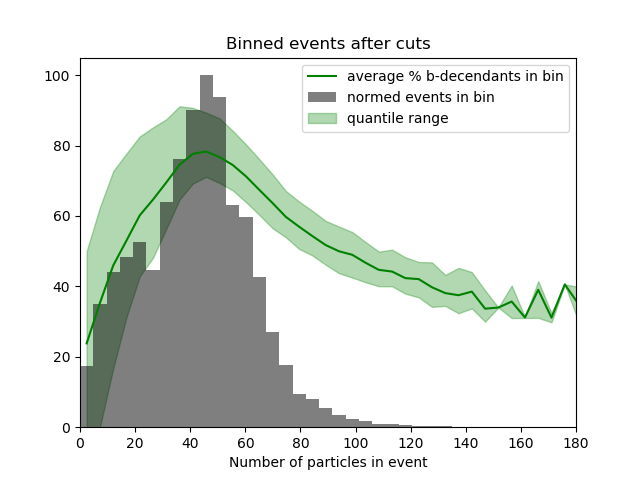
\includegraphics[width=1\textwidth]{graphics/binned_events.png}
    %    \end{minipage}\hfill
    %    \begin{minipage}[c]{0.45\textwidth}
    %        \caption{The end state particles in the simulated events are filtered
    %            with the standard cuts, \(p_T > 0.5\), \(|\eta| < 2.5\).
    %            The events are binned according to how many particles remain after the cuts.
    %            The percentage of \bthing{descendants} in the remaining event after the cuts
    %            is averaged for each bin and plotted on the same axis.
    %            After the cuts have been applied most events are left with around \(50\) particles.
    %                 The percentage of particles that are descendant from a \bthing{quark} varies,
    %                 it is at its highest in events with \(50\) particles,
    %             and most variable in events will small multiplicity.
    %            Very large and very small events tend to be mostly background,
    %            mid sized events are mostly signal.
    %         }\label{fig:bdecendantpercent}
    %    \end{minipage}
    %\end{figure}    
    %
    %
    %\begin{figure}[htp]
    %    \begin{minipage}[c]{0.5\textwidth}
    %        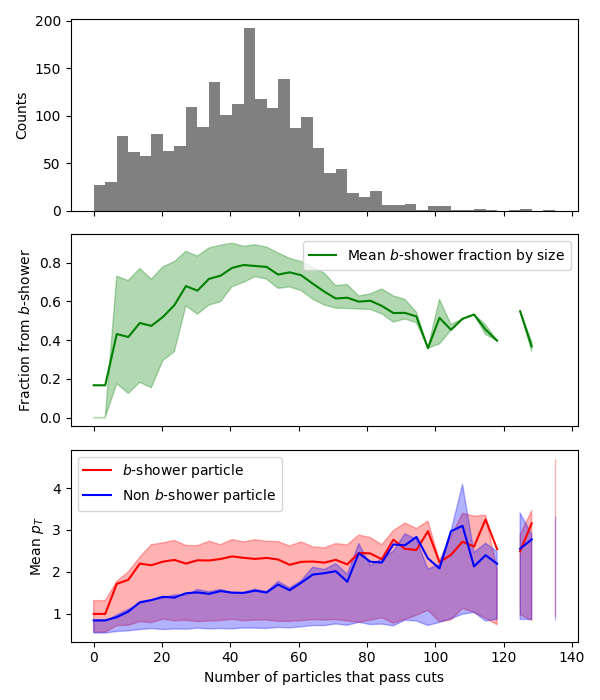
\includegraphics[width=1\textwidth]{graphics/event_composition.png}
    %    \end{minipage}\hfill
    %    \begin{minipage}[c]{0.45\textwidth}
    %        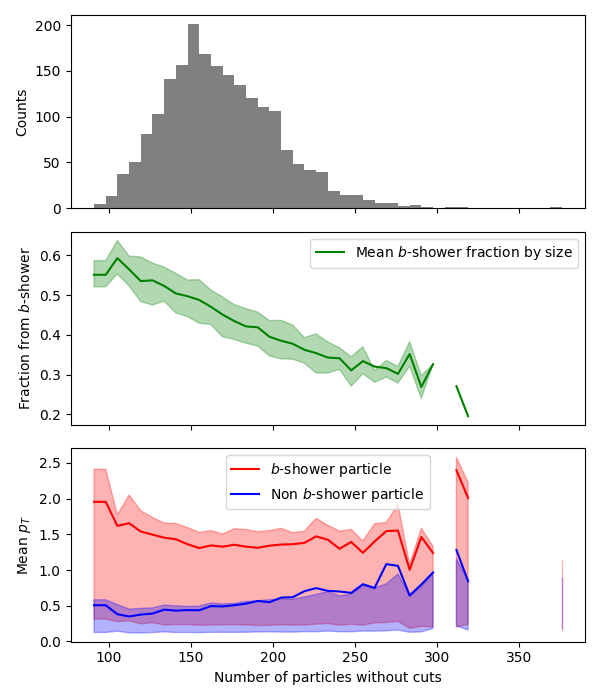
\includegraphics[width=1\textwidth]{graphics/event_composition_nocuts.png}
    %        \caption{Left = with cuts, right = without cuts.
    %         }
    %    \end{minipage}
    %\end{figure}    
    %
    %
    %\begin{figure}[htp]
    %    \begin{minipage}[c]{0.5\textwidth}
    %        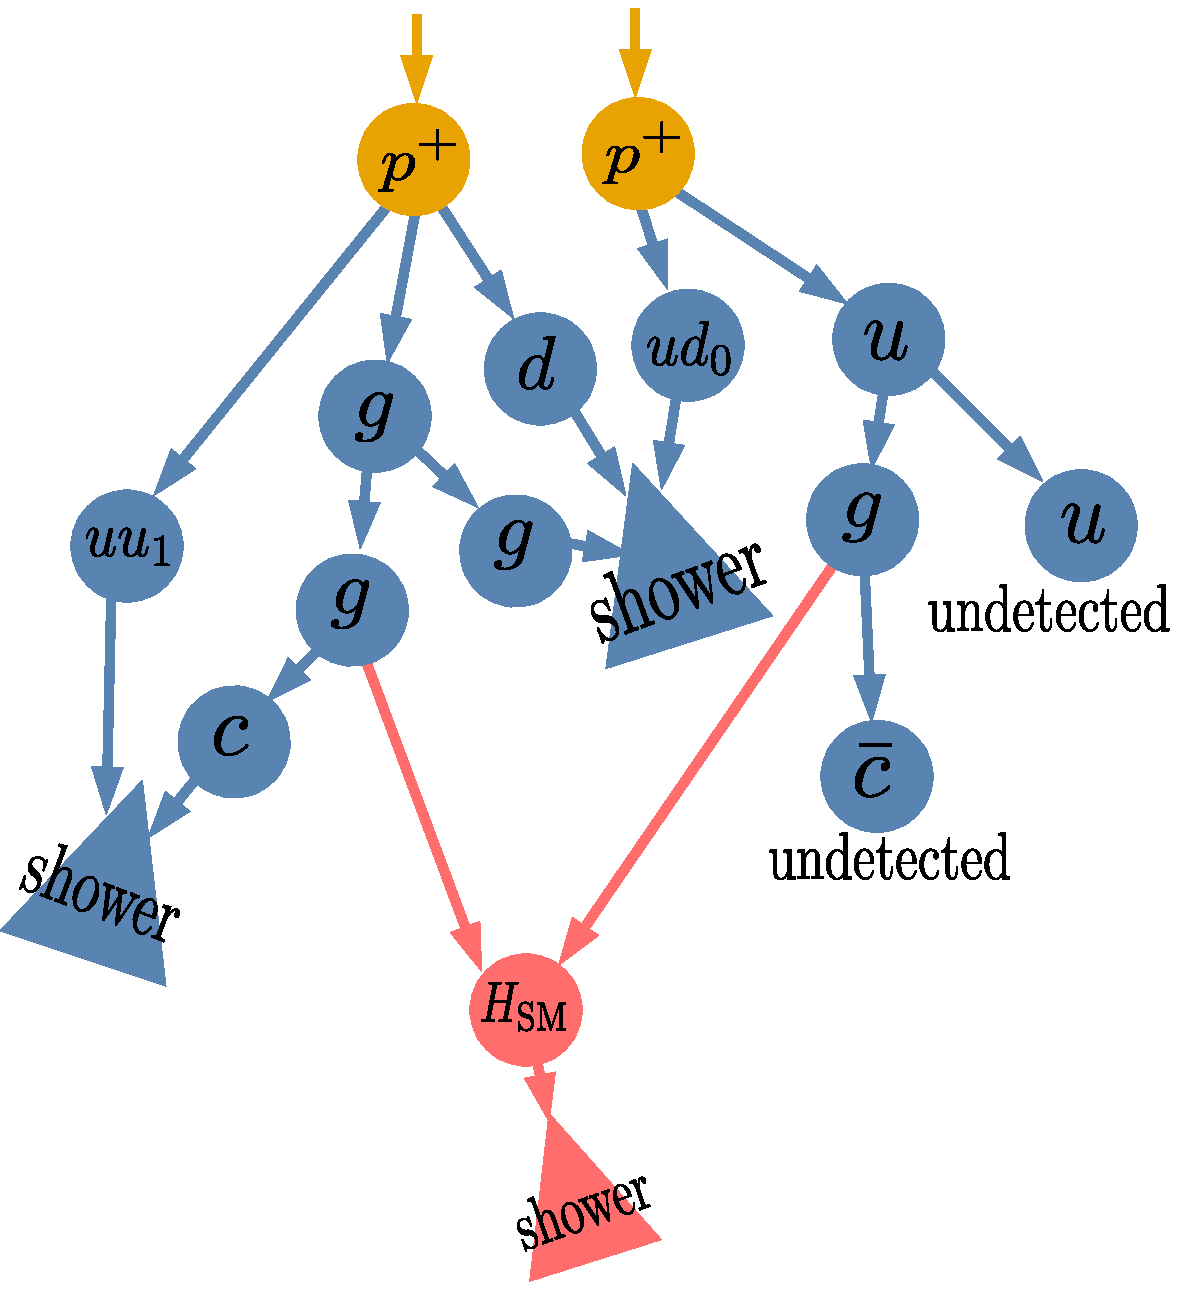
\includegraphics[width=1\textwidth]{graphics/event6.pdf}
    %    \end{minipage}\hfill
    %    \begin{minipage}[c]{0.45\textwidth}
    %        \caption{Drawing of initial state radiation of the 6th even in the dataset.
    %                 The Monte Carlo simulation considers multiple interactions in each vertex,
    %                 and so vertices should eb seen as the combination of multiple steps.
    %                 The information displayed here is what is recorded in the \lstinline{.hepmc} file
    %                 produced by \lstinline{Delphes}.
    %                 A gluon coming from the \(u\) in the left proton producing radiation (the \(c\) and \(g\)) leads to detectable showers.
    %                 The up quark from the right hand proton would have created a shower, but the shower is undetected, either due to high rapidity or low \(p_T\).
    %             Showers are often contributed to from many parts of the initial state radiation, so attributing them has some ambiguity.}
    %        \label{fig:isr}
    %%        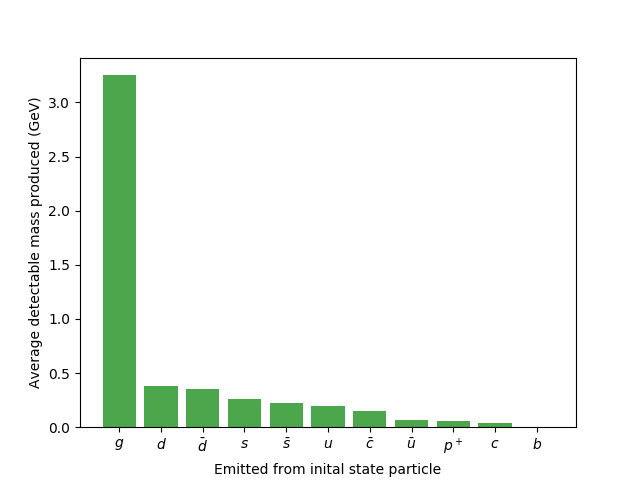
\includegraphics[width=1\textwidth]{graphics/initalstaterdiation_sources.png}
    %%        \caption{In the plot the energy of the initial state particle is used to guess its contribution to the mass of the resulting shower.
    %%            This is done after detector cuts (particle \(p_T > 0.5\) and \(|\text{rapidity}| < 2.5\))
    %%        Taking this rule, on average each event has about \(3\)GeV worth of radiation from initial state gluons.
    %%        Other initial state particles contribute smaller amounts of radiation.}
    %%                 
    %    \end{minipage}
    %\end{figure}    
    %A particle is considered a \bthing{descendant} if it is found in the chain of decays from a \bthing{quark},
    %as opposed to decaying from the ISR.
    %Exactly how the percentage of \bthing{descendants} changes with event size is visualised in figure~\ref{fig:bdecendantpercent}.

\subsection{Determining IRC safety}\label{sec:IRCmethod}
    It would be possible to demonstrate IRC safety analytically, however,
    as the environment required for clustering on Monte Carlo data is already set up
    it is more efficient for this study to prove IRC safety with data.
    This can be done by showing that an IRC sensitive variable, for example the jet mass spectrum,
    is stable between a leading order (LO) dataset with no IRC singularities and a next to leading order (NLO)
    dataset which will contain IRC singularities.

    Showing the jet mass spectrum at LO and NLO for a particular configuration,
    that is a particular selection of clustering parameters,
    would allow a comparison that would highlight any differences cause by IRC sensitivity.
    This will be done for illustrative purposes,
    however, event an IRC unsafe algorithm such as Iterative Cone~\cite{cacciari_antikt2018}
     has some configurations for which it these singularities are avoided.

    To provided a more global view a scan of parameter configurations must be compared.
    Thus, for an unsafe algorithm (such as Iterative Cone) the unsafe configuration
    will be found.
    It would be cumbersome to compare all these jet mass spectrum by eye, however.
    Instead we introduce a summery statistic representing the divergence between two distributions,
    the Jenson Shannon score~\cite{jensen_shannon}.

    The Jenson Shannon score is a value computed between two distributions that increases in magnitude the more these distributions differ.
    It is a symmetrized variant of the Kullback-Leibler divergence.
    The Kullback-Leibler divergence between probability densities \(p\) and \(q\) can be written;
    \begin{equation}
    D_\text{KL} (p | q) = \int^{\inf}_{-inf} p(x) log\left(\frac{p(x)}{q(x)}\right) dx.
\end{equation}
    From which the Jenson Shannon divergence can be written;
    \begin{equation}
    D_\text{JS}(p, q) = \frac{1}{2}D\left(p | \frac{1}{2}(p + q)\right) + \frac{1}{2}D\left(q | \frac{1}{2}(p + q)\right)
\end{equation}
    \(D_\text{JS}\) treats \(p\) and \(q\) symmetrically, and will grow as they become more different.
    The spectrum of Jenson Shannon scores will be plotted for a known IRC safe clustering algorithm, \antikt{},
    a known unsafe clustering algorithm Iterative Cone and the \spectral{} algorithm.

    One small issue with this method is that a large \(D_\text{JS}\) would not differentiate
    between a change in \(p\) and \(q\) due to IRC sensitivity and 
    a change due to noise in the jet mass spectrum.
    The more events used to find the jet mass spectrum the lower the expected noise,
    however is is also possible to subsample within a distribution (LO or NLO)
    to discover how much \(D_\text{JS}\) is influenced by noise.
    If two random sets of jet masses, from events \(a\) and events \(b\) are drawn from the LO events,
    and a \(D_\text{JS}(a, b)\) is computed between them, a large value will indicate that 
    noise in the spectrum is increasing the size of \(D_\text{JS}\) between the LO and NLO spectrums.
    To account for this a subsampled \(D_{JS}\) can be constructed;
    \begin{equation}
    D_{JS, subsampled}(p, q) = \frac{cD_{JS}(p, q)}{\sum_{a \in p, b \in p} D_{JS}(a, b)\sum_{c \in q, b \in q} D_{JS}(c, d)}
\end{equation}
    If this does not differ too much from \(D_{JS}\) then the data sets are large enough the noise in
    the spectrum is not influencing the results.
